\documentclass[a4paper,11pt]{article}
\usepackage{amsmath,amsthm,amssymb}
\usepackage[utf8]{inputenc}
\usepackage[english,russian]{babel}
\usepackage[export]{adjustbox}
\usepackage{graphicx}
\usepackage{pgfplots}
\usepackage{textcomp}

\graphicspath{{pictures/}}
\DeclareGraphicsExtensions{.pdf,.png,.jpg}
\leftskip=-0cm 
\rightskip=-0cm
\voffset = -3cm
\hoffset = -3cm
\textwidth = 550pt
\textheight = 770pt
\pgfplotsset{width=10cm,compat=1.9}


\begin{document}
\Large
HW6
\\
1

\begin{center}
\center{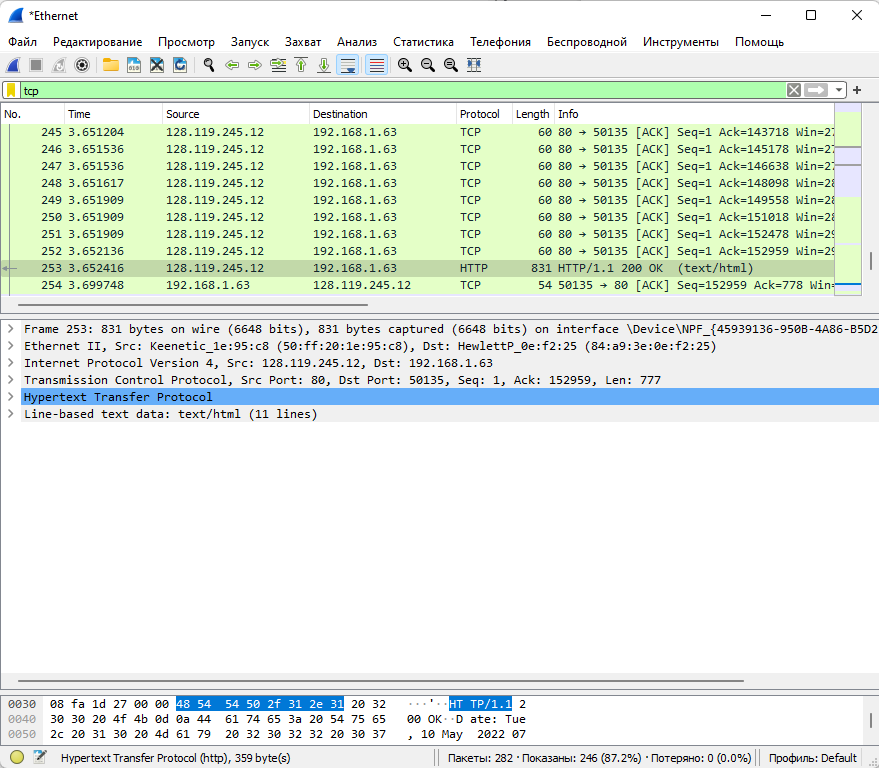
\includegraphics[width =\textwidth]{screenshots/1.png}}
\label{fig:image}
\end{center}
IP адрес компьютера 192.168.1.63, порт 50135

IP адрес сервера 128.119.245.12, порт 80

\begin{center}
\center{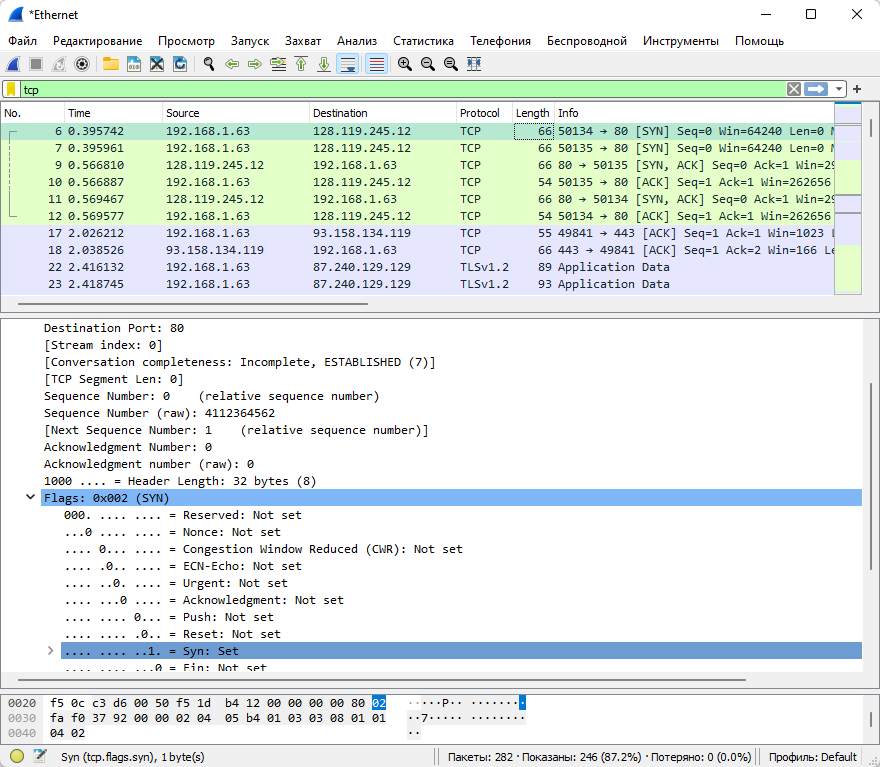
\includegraphics[width =\textwidth]{screenshots/2.png}}
\label{fig:image}
\end{center}
Sequence Number: 0    (relative sequence number)

Sequence Number (raw): 4112364562

По флагу можно определить, что это SYN-сегмент: Flags: 0x002 (SYN)

\begin{center}
\center{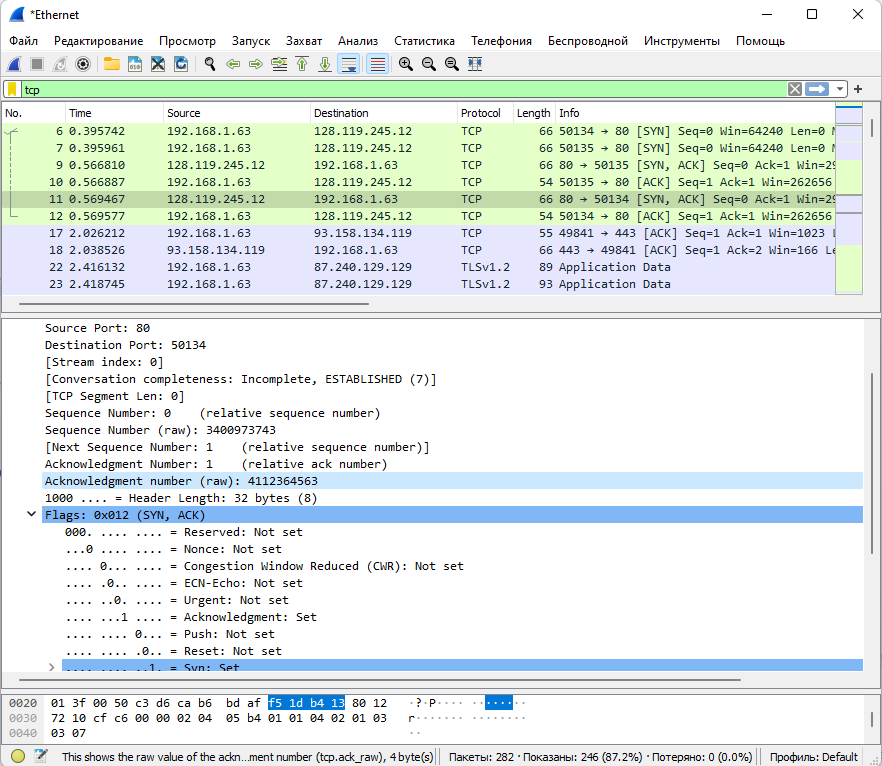
\includegraphics[width =\textwidth]{screenshots/3.png}}
\label{fig:image}
\end{center}
Sequence Number: 0    (relative sequence number)

Sequence Number (raw): 3400973743

Acknowledgment number (raw): 4112364563 = Sequence Number (raw): 4112364562 + 1

По флагу: Flags: 0x012 (SYN, ACK)

\begin{center}
\center{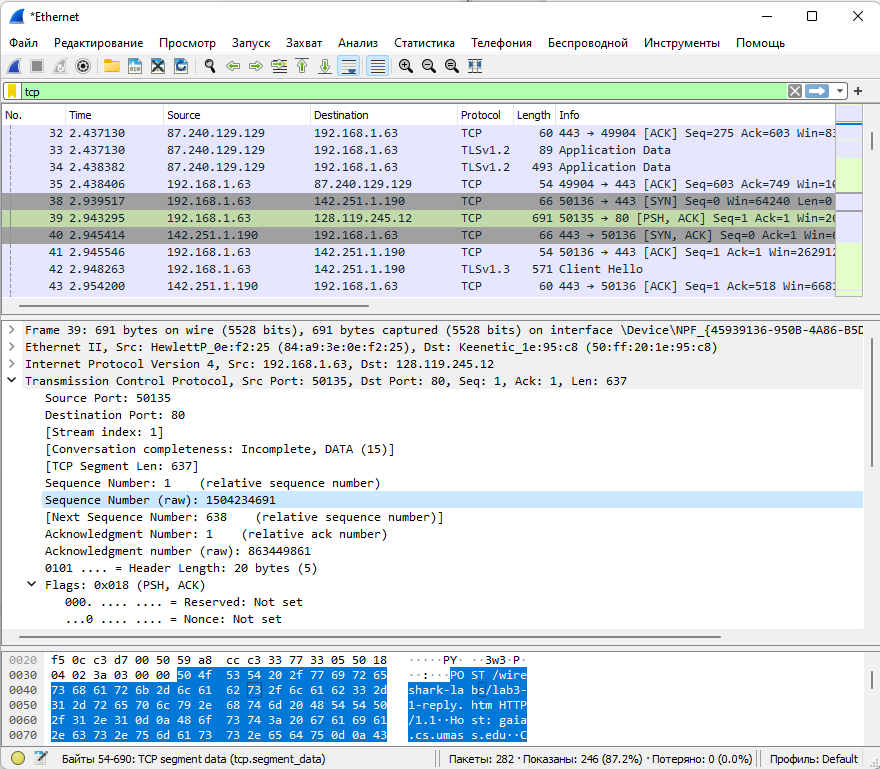
\includegraphics[width =\textwidth]{screenshots/4.png}}
\label{fig:image}
\end{center}
Sequence Number: 1    (relative sequence number)

Sequence Number (raw): 1504234691

\begin{center}
\center{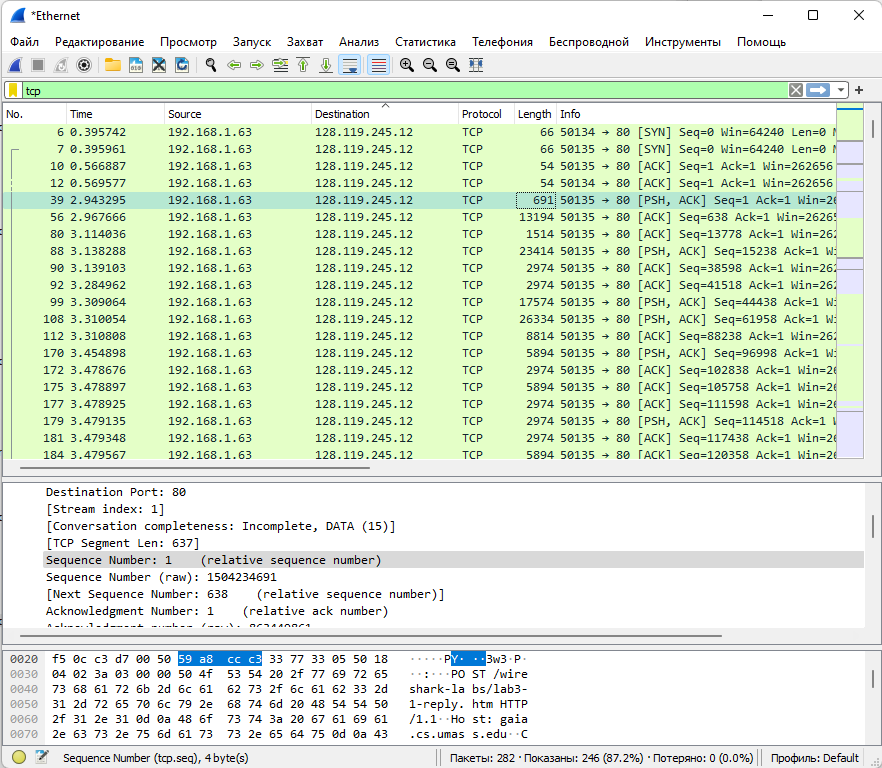
\includegraphics[width =\textwidth]{screenshots/5.png}}
\label{fig:image}
\end{center}
Номера:\\
Sequence Number: 1    (relative sequence number), Sequence Number (raw): 1504234691\\
Sequence Number: 638    (relative sequence number), Sequence Number (raw): 1504235328\\
Sequence Number: 13778    (relative sequence number), Sequence Number (raw): 1504248468\\
Sequence Number: 15238    (relative sequence number), Sequence Number (raw): 1504249928\\
Sequence Number: 38598    (relative sequence number), Sequence Number (raw): 1504273288\\
Sequence Number: 41518    (relative sequence number), Sequence Number (raw): 1504276208

Время на скрине, первый 2.943295, последний 3.284962	

\begin{center}
\center{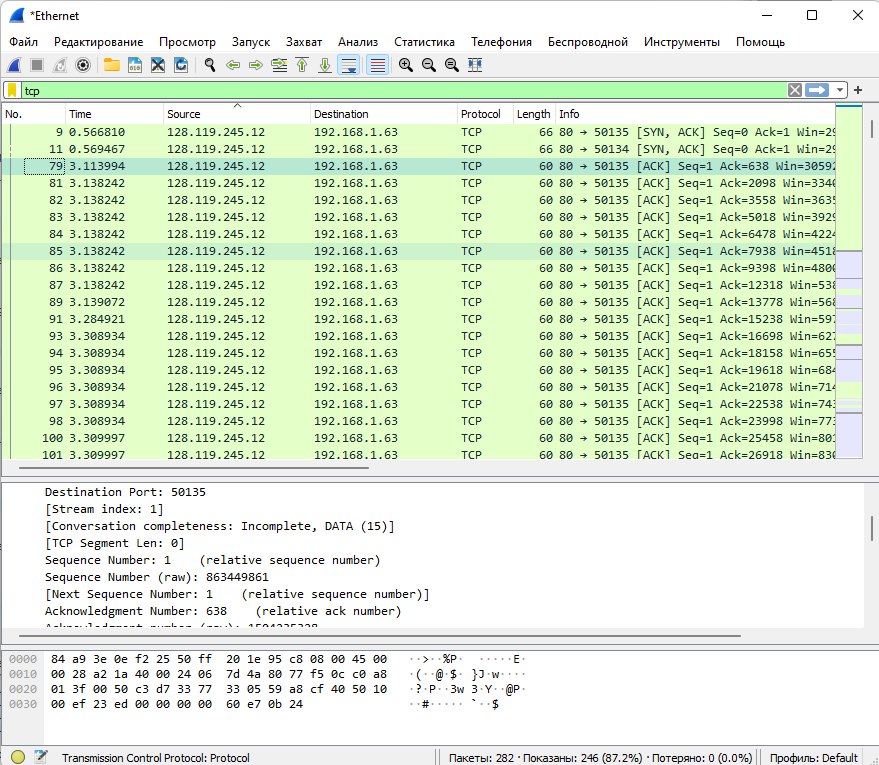
\includegraphics[width =\textwidth]{screenshots/6.png}}
\label{fig:image}
\end{center}

\begin{center}
\center{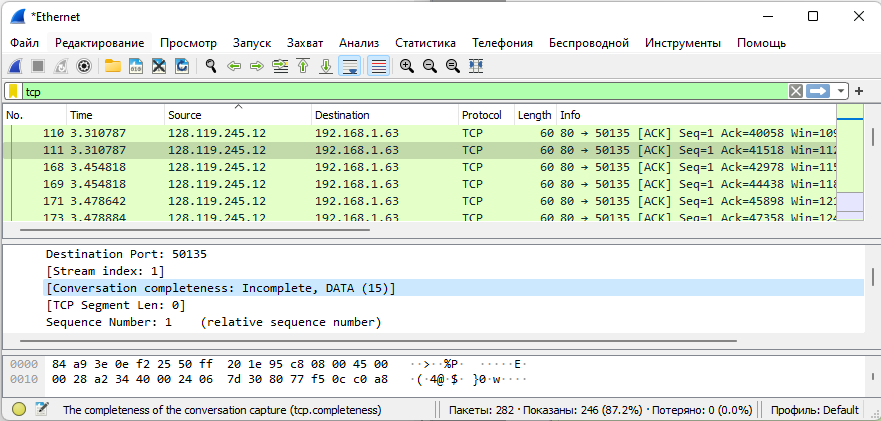
\includegraphics[width =\textwidth]{screenshots/7.png}}
\label{fig:image}
\end{center}
Чтобы определить ответное подтверждение, надо сравнить Ack полученного и Seq отправленного

Время получения первого 3.113994, второго 3.139072, последнего 3.310787

\begin{center}
\center{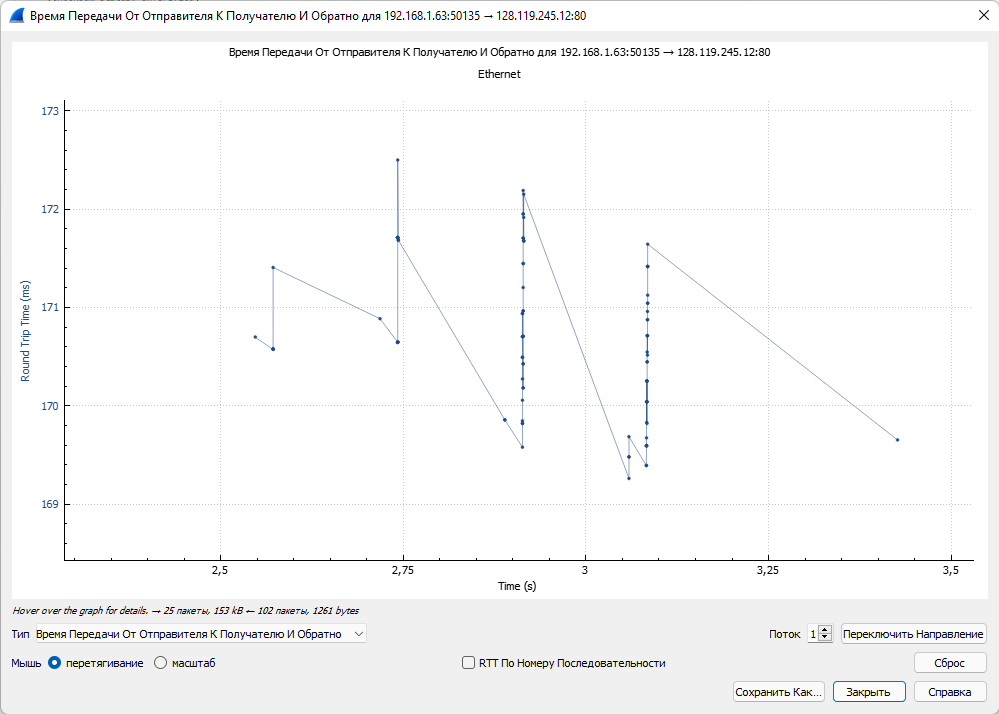
\includegraphics[width =\textwidth]{screenshots/8.png}}
\label{fig:image}
\end{center}
Для подсчета RTT можно посмотреть на разность времени получения и времени отправки, это также можно видеть на графике. Для первых 6 точек значение между 170 и 173 мс

\begin{center}
\center{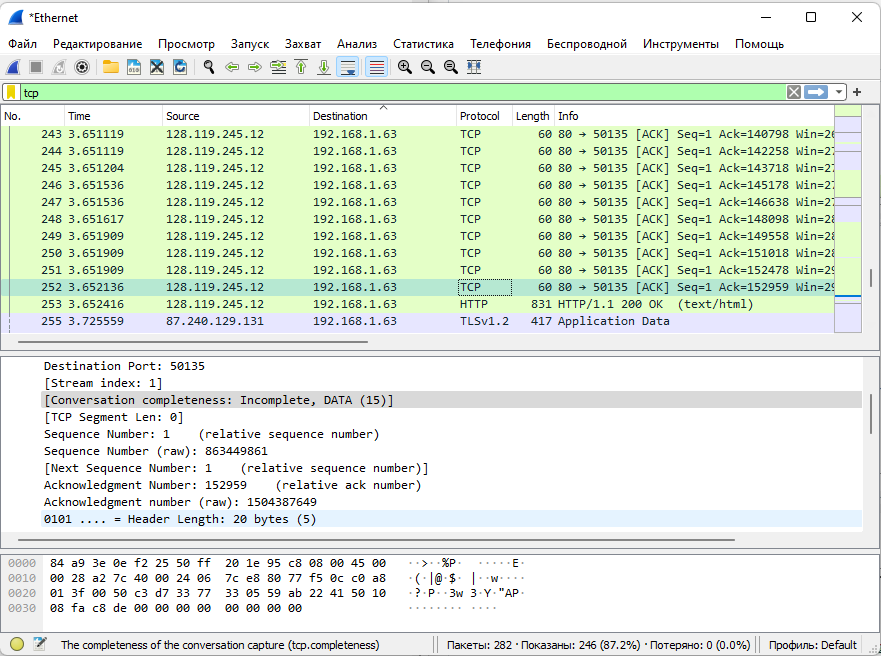
\includegraphics[width =\textwidth]{screenshots/10.png}}
\label{fig:image}
\end{center}
Время отправки первого SYN 0.395742, получения последнего ACK 3.652136, размер данных 152138 байт. Тогда пропускная способность 
$$\frac{152138}{(3.652136 - 0.395742)} = 46719 \text{ байт/с}$$

\newpage
2
\begin{center}
\center{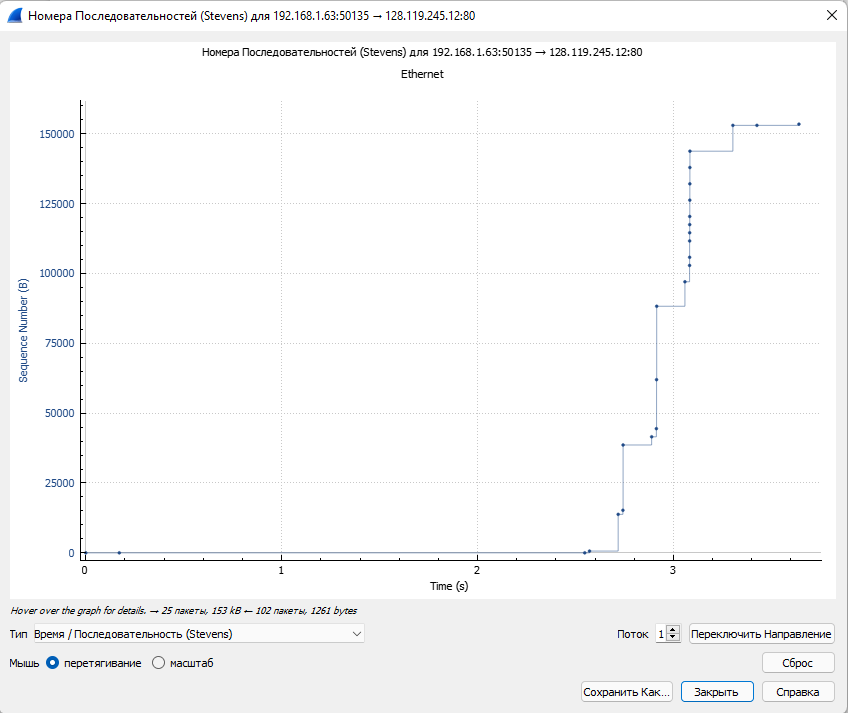
\includegraphics[width =\textwidth]{screenshots/9.png}}
\label{fig:image}
\end{center}
\end{document}








































